% Datensammlungsprozess
% inklusiv: wohin? wie? welche Daten und welche Techniken benutze ich?
% und Die Ergebnisse
% stelle die Datensstruktur vor, welche Geschlechtsituation, Scale von Verkaufen
% ===========================================================
\chapter{Datensammlung und Textverarbeitung} \label{datensammlung}
% ===========================================================
%
Die Kommentaren auf deutschen und chinesischen Webseiten für die gleichen Produkte von sportlichen Kleidungen werden in dieser Arbeit gesammelt. 
Die chinesischen Kommentaren werden durch eine Übersetzungsmaschine (Google Translate) ins Deutsche übersetzt. Die Einflüsse von den Übersetzungen auf die Ergebnisse, besonders wegen der Ungenauigkeit von Übersetzungsmaschine, werden im Abschnitt \ref{mehrsprachig} diskutiert. 
\section{Datenquellen}
% ===========================================================
%
Die deutsche Daten werden aus Amazon.de gesammelt, und die chinesische aus Tmall.com. Die beiden sind die wichtigsten \acs{B2C} Plattformen in den jeweiligen Ländern.
%% \todo[inline]{stelle die beiden Datenquellen (sowie beiden Vertriebsplatformen)vor. Suchen einige Quelle zu unterstützen}
% =======================================================
\subsection{Amazon weltweit und in Deutschland}
% =======================================================
Amazon ist präsent auf den derzeit größten E-Commerce-Märkten weltweit und bietet einen schnellen und einfachen Zugang zu diesen. \href{http://www.amazon.de}{Amazon.de}, die deutschsprachige Website, wird von der Amazon.com, Inc. betrieben. Die Amazon.com, Inc. ist ein amerikanischer Online-Versandhändler mit einer breit gefächerten Produktpalette. Vom Zeitpunkt des Debüts von Amazon.com als Webseite im Juli 1995 bis Anfang 1999 hat Amazon.com Inc. eine Marktkapitalisierung von {\$}6 Milliarden erreicht, das ist mehr als Barnes{\&}Noble und Borders, die größten Rivalen on-und offline, zusammen. Im Letzten Quartal von 1998 beliefen sich die Internetverkäufe auf {\$}252,9 Millionen, das ist ein 283{\%}iger Zuwachs über den Nettoumsatz von {\$}66 Millionen im letzten Quartal von 1997.\citep[p.~15]{saunders2001amazon}\\
\begin{figure}[htb]
	\begin{center}
		
\includegraphics[scale=1.0]{datensammlung/logo_amazon}
		\caption[Logo von Amazon Deutschland]{Logo von Amazon Deutschland(Quelle:\href{http://www.amazon.de}{Amazon.de})}
		\label{fig:logo_amazon}
	\end{center}
\end{figure}\\
Nach dem Geschäftsbericht im Jahr 2014 von der amerikanischen Börsenaufsicht (\ac{SEC}), hat die Amazon.com, Inc. einen Nettoveräußerungserlös von {\$}88.988 Millionen\citep{Amazon2014}. Abbildung \ref{fig:UmsatzerloeseAmazonCom} zeigt das Wachstum der Umsatzerlöse von Amazon.com, Inc. von 2010 bis 2014.\\
\begin{figure}[htb]
	\begin{center}
		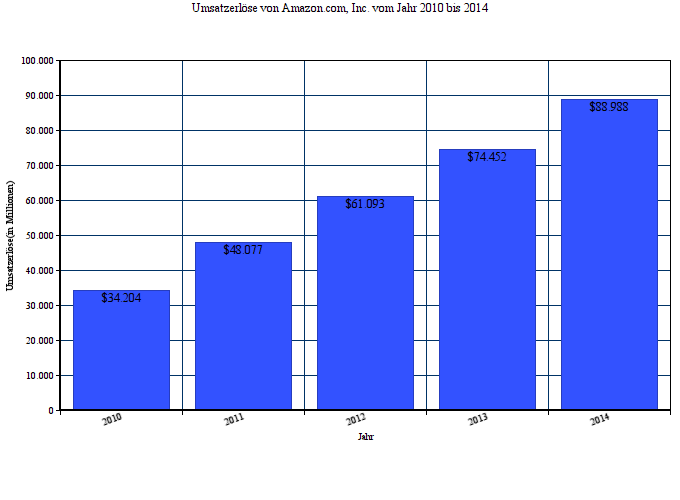
\includegraphics[width=\textwidth]{datensammlung/Umsatzerloese_Amazon_com}
		\caption[Umsatzerlöse von Amazon.com]{Umsatzerlöse (US Dollar in Millionen) von Amazon.com, Inc. 2010 - 2014 (Datenquelle:\citealp{Amazon2014,Amazon2013})}
		\label{fig:UmsatzerloeseAmazonCom}
	\end{center}
\end{figure}\\
Für Amazon.com, Inc. ist Deutschland der umsatzstärkste Auslandsmarkt\citep{onlineHandel2013}. Deutschland stand im Jahr 2014 für 13 Prozent des Gesamtumsatzes von Amazon, und im Jahr 2013 für 14 Prozent\citep{Amazon2014}. Der Bundesverband des Deutschen Versandhandels hat den Gesamtumsatz des deutschen Online-Handels im vergangenen Jahr auf 27,5 Milliarden Euro beziffert. Zahlen des Einzelhandelsverbands sprechen von einem Umsatz von 29,5 Milliarden Euro. Demnach kontrolliert Amazon ein gutes Fünftel oder sogar fast ein Viertel des gesamten deutschen Online-Versandhandels.\citep{onlineHandel2013} Abbildung \ref{fig:UmsatzerloeseAmazonDe} zeigt das starke Wachstum des Erlöses vom Deutschland-Geschäft ab 2010 bis 2014.\\
\begin{figure}[htb]
	\begin{center}
		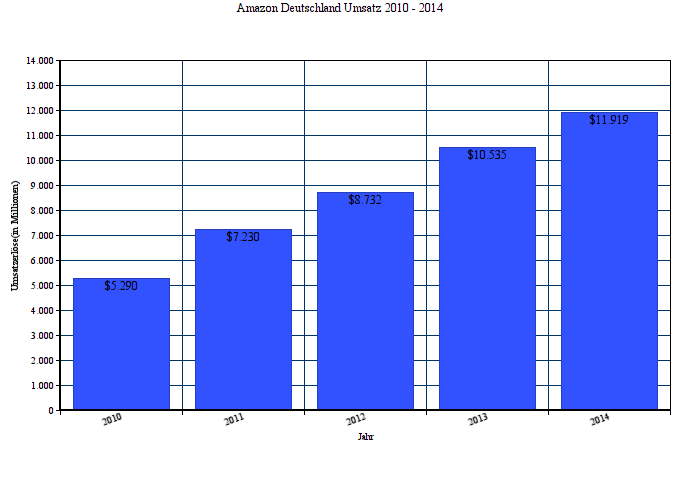
\includegraphics[width=\textwidth]{datensammlung/Umsatzerloese_Amazon_de}
		\caption[Amazon Deutschland Umsatz 2010-2014]{Amazon Deutschland Umsatz 2010 - 2014 (US Dollar in Millionen) (Datenquelle:\citealp{Amazon2014,Amazon2013})}
		\label{fig:UmsatzerloeseAmazonDe}
	\end{center}
\end{figure}\\
Mehrere internationale Textilhersteller sind über Amazon Deutschland aufgelistet, \acs{bzw.} Adidas, Nike, Puma und so weiter. Deshalb ist Amazon Deutschland ein gutes Objekt im Bereich elektronischer Textileinzelhandel zu studieren.
\subsection{Chinesische Plattform:``Tmall''}
% =======================================================
\href{http://www.tmall.com}{Tmall.com} ist eine chinesischsprachige Webseite für \acs{B2C} Online-Einzelhandel, die sich im Jahr 2008 von \href{http://www.taobao.com}{Taobao.com} aufgespalten hatte. Es ist das größte Plattform für lokale chinesische und internationale Unternehmen, um Markenware für die Verbraucher in der Volks Republik China, Hongkong, Macao und Taiwan zu verkaufen.
\begin{figure}[htb]
	\begin{center}
		
\includegraphics[scale=0.5]{datensammlung/logo_tmall}
		\caption[Logo von Tmall.com]{Logo von Tmall.com(Quelle:\href{http://www.tmall.com}{Tmall.com})}
		\label{fig:logo_tmall}
	\end{center}
\end{figure}
Im Jahr 2013 wurde Tmall das größte Open-Portal für Online Händler und Endverbraucher, mit einem Anteil am chinesischen Online-Markt ca.50{\%}.\citep{CECRC2014a}
Tabelle \ref{table:markt_anteil_in_china} zeigt fast alle Online Händler in der chinesischen Online-Marktposition.\\

\begin{table}[htb]
	\centering
	\begin{tabular}{|c|c|}
	\hline
	Online Händler & Marktanteil({\%})\\
	\hline
	Tmall & 50,1\\
	JD.com & 22,4\\
	Suning.com & 4,9\\
	Tecent B2C & 3,1\\
	Amazon China & 2,7\\
	Yihaodian & 2,6\\
	Vipshop & 2,3\\
	Dangdang & 1,4\\
	Gome & 0,4\\
	\hline
	\end{tabular}
	\caption[Marktpositionen von Online Händler in China]{Marktpositionen von Online Händler in China.(Quelle: \citealp{CECRC2014a})}
	\label{table:markt_anteil_in_china}
\end{table}

Mit mehr als 10 Millionen jährlich aktiven Anbieter und über 140.000 Marken in Tmall bis zum 31. März 2015 bieten die Marktplätzen von Tmall den Verbraucher wettbewerbsfähige Preisgestaltung in einer breit angelegten Skala von Kategorien. Wegen der Anwesenheit einer großen Anzahl von globalen Marken und den hohen Anforderungen an die auf Tmall betriebenen Händlern, hat sich eine Präsenz auf Tmall zu einer Validierung der Qualität, um die Händler die Markenbekanntheit zu bauen und erweitern. Gleichzeitig ist Tmall eine vertrauenswürdige Plattform für die chinesischsprachigen Verbraucher, um sowohl einheimische als auch internationale Markenprodukte zu kaufen, selbst wenn Produkte nicht verfügbar in den traditionellen Verkaufsstellen sind.\citep{Alibaba2014}

Tmall ist zum Synonym für Online-Shopping in China geworden. Die Verbraucher kommen auf die Plattform mit starken kommerziellem Absicht, die zu hohen Umsätze für die Händlern führt. Abbildung \ref{fig:tmall_gmv} zeigt das Wachstum der \ac{GMV} von Tmall ab 30. Juni 2013 bis 31. März 2015.\citep{Alibaba2014} Wegen dem großen Erfolg in China ist Tmall als eine gute Plattform für den chinesischen Online-Handel zu studieren.
 
\begin{figure}[htb]
	\begin{center}
		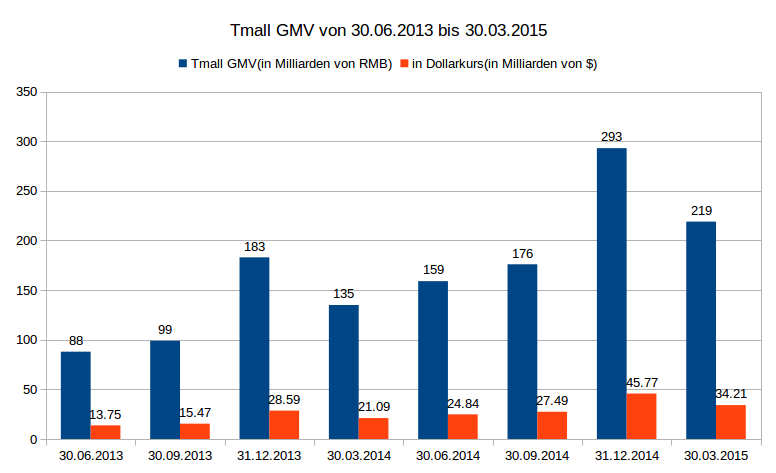
\includegraphics[scale=0.56]{datensammlung/Tmall_GMV}
		\caption[Tmall \acs{GMV}]{Tmall \ac{GMV} von 30.06.2013 bis 30.03.2015 (Datenquelle:\citealp{Alibaba2014})}
		\label{fig:tmall_gmv}
	\end{center}
\end{figure}
%%=========================================================
\section{Online Textileinzelhandel in den beiden Ländern} \label{sec:online_kleidung}
%%=========================================================
Dieser Abschnitt stellt die Situationen des Markts von Online Textileinzelhandel in Deutschland und China vor. Diese Vorstellung ist wichtig, man diese Situationen zu wissen, um die Arbeit besser zu verstehen.

Mit mehr als 51 Millionen (94 Prozent der Internetnutzer ab 14 Jahren) digitale Verbraucher im Jahr 2014, genießt Deutschland die größte E-Commerce-Kundenpotenzial in Europa - und ist damit der klare kontinentale Führer \citep{Spath2015}. In ``The 2015 Global Retail E-Commerce Index'' ist Deutschland am fünfth Position \citep{HanaBen-Shabat2015}. 

Kleidung, Elektronische Waren und Bücher gehören zu den beliebtesten Online-Kategorien. 88 Prozente der Befragter sagen, dass sie in den letzten drei Monaten Kleidungen online gekauft haben, während der Weltdurchschnitt 76\% ist. \citep{HanaBen-Shabat2015}

Und die Kategorie ``Bekleidung, Textilien und Schuhe'' hat eine der stärksten Wachstumsraten für den Zeitraum 2011-2014. Die höchsten Umsätze im E-Commerce werden in der Produktkategorien Bekleidungs (11,9 Mrd. EUR), Unterhaltungselektronik (5 Mrd. EUR) und Bücher (4,1 Mrd. EUR) generiert. Als die Abbildung \ref{fig:kleidung_de} gezeigt, werden 42\% Kleidungen in Deutschland online verkauft. \citep{Spath2015} 

\begin{figure}[htb]
	\begin{center}
		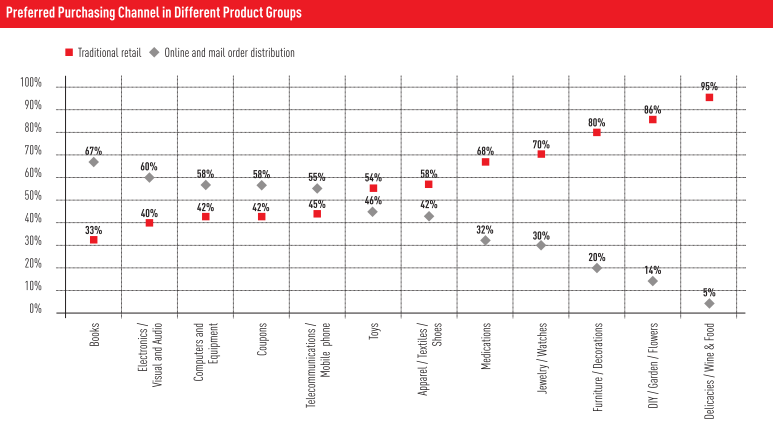
\includegraphics[width = \textwidth]{datensammlung/kleidung_de}
		\caption[42\% Textilien werden in Deutschland online verkauft]{42\% Textilien werden in Deutschland online verkauft(Quelle:\citealp{Spath2015})}
		\label{fig:kleidung_de}
	\end{center}
\end{figure}

China, das weltweit bevölkerungsreichsten Land (fast 1,4 Milliarden Menschen), ist online aktiv. Mehr als ein Drittel der Menschen, die online mindestens einmal pro Woche surfen, sind "ständig verbunden", und 58 Prozenten prüfen das Internet zwei bis vier Mal pro Tag. Verglichen mit Deutschland, ist China am zweiten Position in ``The 2015 Global Retail E-Commerce Index'', nur nach den USA.\citep{HanaBen-Shabat2015}

\begin{figure}[htb]
	\begin{center}
		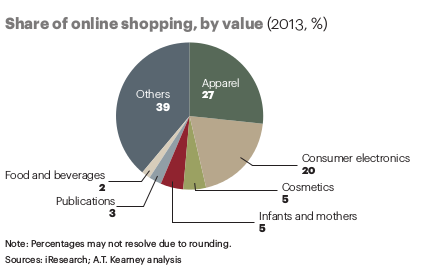
\includegraphics[scale =1.0]{datensammlung/anteil_kleidung_cn}
		\caption[Anteil der Online-Shopping in China]{Anteil der Online-Shopping in China, nach Wert (2013, \%)(Quelle:\citealp{goh2014china})}
		\label{fig:anteil_kleidung_cn}
	\end{center}
\end{figure}

Online-Handel ist die am schnellsten wachsende Einzelhandels für Bekleidung in China \citep{fung2014china}. Abbildung \ref{fig:anteil_kleidung_cn} stellt fest, dass 27\% des Umsatzes in 2013 durch Kleidung verkauft werden, größer als die Kategorie Unterhaltungselektronik. Wie die Abbildung \ref{fig:kleidung_cn} gezeigt, wuchs die gesamte Online-Bekleidungs-Transaktionswert in China deutlich um 42,6\% gegenüber dem Vorjahr um 434,9 Milliarden Yuan (62,1 Milliarden Euro) im Jahr 2013 zu erreichen \citep{fung2014china}.

``Kleidung, Schuhe, Hüte, Taschen und Koffer, Outdoor-Produkte'' sind die beliebtesten Kategorien in Online-Shopping im Jahr 2013 erworben, und diese Kategorie wird von 41,3\% der Frauen und 28\% der Männer inzwischen Top 10 Lieblings Waren in Online-Shopping gewählt \citep{fung2014china}. 97\% der Befragter sagen, dass sie in den letzten drei Monaten Kleidungen online gekauft \citep{HanaBen-Shabat2015}.

\begin{figure}[htb]
	\begin{center}
		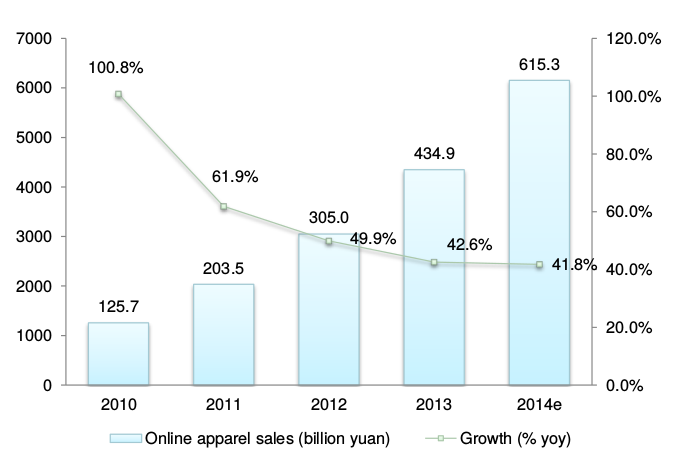
\includegraphics[width=\textwidth]{datensammlung/kleidung_cn}
		\caption[Online Umsatz für Kleidung in China]{Online Umsatz für Kleidung in China, 2010 - 2014(Quelle:\citealp{fung2014china})}
		\label{fig:kleidung_cn}
	\end{center}
\end{figure}
%%=========================================================
\section{Sportkleidung als Untersuchungsobjekt} \label{sec:untersuchungsobjekt}
%%=========================================================
Diese Arbeit macht einen Vergleich über Online-Kommentaren zwischen Deutschland und China im Bereich Textileinzelhandel. Um dieses Ziel zu erreichen, sollen die Studienobjekte folgende Bedingungen erfüllen:
%%===============================
\begin{enumerate}
	\item Die Studienobjekte sollten Kleidung oder Textilien sein.
	\item Die Studienobjekte sollten in Deutschland und China im Internet verkauft werden.
	\item Die Studienobjekte sollten auf den gewählten Plattformen (Amazon.de und Tmall) viele Kommentaren haben.
	\item Jedes ausgewählte Studienobjekt sollt in den beiden Ländern gleich sein.
	\item Es sollte keine Fashion-Elemente geben.
\end{enumerate}
%%================================
Bedingung 1 beschränkt die Arbeit im textilen Bereich, und die Bedingung 2 und 3 werden es einem möglich machen die Online-Kommentaren zu analysieren. Mit der Erfüllung der vierten Bedingung macht der Vergleich akademischen und geschäftlichen Sinn, weil es große Änderungen in einem Zeitraum über Fashion gibt, und dazu Fashion ein ganz anderes Thema ist, wird diese Arbeit die Fashion-Elemente von den Kleidungen rausnehmen.
 Es gibt noch eine potenzielle Bedingung: Alle Studienobjekte sollten in den beiden Ländern sehr gut verkauft werden, damit sie viele Kommentaren haben.
%%================================

Aufgrund der obigen Bedingungen werden drei internationalen Textilmarken (Adidas, Nike und Puma) aus unterschiedlichen Marken in dieser Arbeit ausgewählt. Alle  drei Marken sind sportliche Artikel, um die Bedingung 5 zu erfüllen.
\begin{itemize}
	\item \textbf{Nike, Inc.} ist ein amerikanischer multinationaler Konzern, die in der Konstruktion, Entwicklung, Produktion und weltweite Vermarktung und Verkauf von Schuhen, Bekleidung, Ausrüstung, Zubehör und Dienstleistungen tätig ist. Nike ist einer der weltweit größten Anbieter von Sportkleidung und Schuhe, und ein bedeutender Hersteller von Sportartikeln, mit einem Umsatz von mehr als 24,1 Milliarden US-Dollar im Geschäftsjahr 2012. Ab 2012 beschäftigt es mehr als 44.000 Mitarbeiter weltweit. Im Jahr 2014 wurde die Marke allein zu 19 Milliarden Dollar geschätzt und ist damit die wertvolle Marke unter den Sport Unternehmen. \citep{mahdi2015comparative} 
	\item \textbf{Adidas AG} mit Sitz in Herzogenaurach ist ein deutscher Sportartikelhersteller mit den Marken Adidas, Reebok und TaylorMade. Seit dem 17. November 1995 ist der Konzern im Deutschen Aktienindex an der Frankfurter Wertpapierbörse notiert und gilt nach Nike als der zweitgrößte Sportartikelhersteller der Welt \citep{langenscheidt2010lexikon}. Es ist ein Haushalts Markte mit den drei Streifen Logo auf den Märkten in der ganzen Welt anerkannt. Das Produktprotfolio des Unternehmens ist groß und reicht von Sportkleidung und Schuhe, und Accessoires wie Taschen, Uhren, Brillen und andere sportbezogene Produkte und Ausrüstung. Adidas beschäftigt mehr als 46.000 Menschen Weltweit. Die Adidas Gruppe besteht aus rund 170 Tochtergesellschaften einschließlich Reebok, Taylormade-Adidas Golf, Rockport und CCM-Hockey. Der Hauptsitz der Gruppe ist in Herzogenaurach, Deutschland. Im dritten Quartal 2014 betrug der Umsatz der Gruppe 4,118 Milliarden Dollar. \citep{mahdi2015comparative}
	\item \textbf{Puma SE} mit Sitz in Herzogenaurach ist ein börsennotierter Sportartikelanbieter und Hersteller von Schuhen, Textilien und Accessoires \citep{peters2007puma}. Puma ist mit rund drei Milliarden Euro Jahresumsatz, einem Konzerngewinn von 5,3 Millionen Euro und 10.982 Mitarbeitern im Jahr 2013 neben Adidas und Nike einer der weltweit größten Sportartikelhersteller (\href{http://about.puma.com/de/this-is-puma/}{About Puma, 2014}).
\end{itemize}
Die drei sind die weltweit größten sportlichen Textilhersteller, und in Deutschland und China verkaufen sie schon lange und gut. Deshalb ist es einfach, die Kleidungen zu finden, die die 5 Bedingungen erfüllen können. In dieser Arbeit werden insgesamt 4 solche Kleidungen als Studienobjekte genutzt. 2 Kleidungen davon sind Hosen und die anderen 2 sind T-Shirt. 3 Kleidungen sind für Herrn und eine für Damen. Die beiden Hosen werden von Adidas hergestellt, eine weibliche und eine männliche. Die beiden männlichen T-Shirts sind jeweils von Nike und Puma.
%%===============================
\section{Technische Werkzeuge für die Datensammlung}
%%\todo[inline]{stelle die Werkzeuge vor: Scrapy, Python, XPath, Google Translate usw.}
\subsection{Datensammlung aus Webseiten mit Python}
%%====================================
Python hat von Data-Miner Gemeinschaft für Datensammlung entweder im Internet oder anderswo als eine perfekte Sprache gewonnen \citep{Khwaldeh2013}. Tools und Methoden von Python können nach der ausgeführten Funktion oder der Klasse der verwendeten Anwendung klassifiziert werden, weil es viele positive Eigenschaften besitzt: \citep[p.~X]{segaran2008kollektive}
\begin{description}
	\item[Kürzer] \hfill \\
	Code, der in dynamisch typisierten Sprachen wie Python geschrieben wird, ist meist kürzer als Code, der in anderen verbreiteten Sprachen entsteht. Das bedeutet, dass einfacher ist, den Algorithmus in Kopf unterzubringen und wirklich zu verstehen, was er tut.
	\item[Leicht zu lesen] \hfill \\
	Python wurde schon als ``ausführbarer Pseudocode'' beschrieben. Das ist natürlich übertrieben, aber es stimmt sehr wohl, dass die meisten erfahrenen Programmierer Python-Code lesen und verstehen können, was er tun soll.
	\item[Einfach erweiterbar] \hfill \\
	Python bringt standardmäßig vielen Bibliotheken mit, unter anderem mit mathematischen Funktionen, zum Parsen von \ac{XML} und zum Laden von Webseiten. Diese Bibliotheken sind frei erhältlich und lassen sich einfach herunterladen, installieren und nutzen.
	\item[Interaktive] \hfill \\
	Wenn man ein Code durcharbeitet, ist es hilfreich, die Funktionen schon auszuprobieren, während man sie schreibt, ohne ein anderes Programm nur zum Testen erstellen zu müssen. Python kann Programme direkt von der Befehlszeile aus ausführen und besitzt zudem einen interaktiven Prompt, an dem man Funktionen startet, Objekte erstellen und Pakete testen könnte.
	\item[Viele Paradigmen] \hfill \\
	Python unterstützt objektorientierte, prozedurale und funktionale Programmierung. Manchmal ist es sinnvoll, Funktionen als Parameter zu übergeben, während man ein anderes Mal den Zustand in einem Objekt ablegt. Python unterstützt beide Vorgehensweisen.
	\item[Viele Plattformen und freie Software] \hfill \\
	Python bietet eine Referenzimplementierung für alle wichtigen Plattformen und ist auf allen frei erhältlich. Der Code, der in dieser Arbeit beschrieben wird, funktioniert unter Windows, Linux und Mac.
\end{description}  
Darüber hinaus kommt Python mit Modulen für den Zugriff auf das Internet wie \emph{urllib} und \href{http://docs.python.org/library/urllib2.html}{\emph{urllib2}}, \href{http://www.clips.ua.ac.be/pages/pattern}{\emph{Pattern}}, \href{http://pypi.python.org/pypi/mechanize/}{\emph{mechanisieren Paket}} und \href{http://scrapy.org}{\emph{Scrapy}}. In dieser Arbeit wird der letzte verwendet, weil Nutzer weniger Zeit und Skript als die anderen benötigt. \citep{Khwaldeh2013}
%%===========================================
\subsection{XPath: Daten Lokalisierung in Webseiten}
%%===========================================
XPath 1.0 gilt als eine Untersprache innerhalb eines \ac{XSLT} 1.0-Stylesheets und ist beim Transformationsprozess unerlässlich. XPath ist also auch unabhängig von \ac{XSLT} nutzbar.
XPath selbst verwendet keine \ac{XML}-Syntax, sondern benutzt Funktionen und Ausdrücke, um XML-Dokumente \acs{bzw.} deren Teile zu adressieren. XPath-Ausdrücke benutzen sogenannte Lokalisierungspfade (Location path), um die gewünschten Knoten im Dokument zu finden. \citep[p.~211-212]{sebestyen2010xml}

Man kann sich solche Lokalisierungspfade wie einen Wegweiser vorstellen: ``\emph{Sie sind jetzt hier und jetzt müssen Sie die Treppe nach unten nehmen, dort nach links und dann die dritte Tür.}'' Der XPath-Ausdruck ``\code{/buch/autor/nachname}'' selektiert das \code{<nachname>} Element im \code{<autor>} Element, das sich unterhalb des \code{<buch>} Element befindet. \citep[p.~212]{sebestyen2010xml}

Mit XPath kann man einfach die gewünschten Daten in Webseiten finden und lokalisieren. Und in Python und Scrapy gibt es noch viele Bibliotheken, die XPath gut unterstützen. Deshalb ist XPath in dieser Arbeit eine wichtige Maßnahme, um die Kommentaren in den Webseiten zu bekommen.  
%%==================================
\subsection{Reguläre Ausdrücke: Bearbeitung der Texte}
%%=================================
Reguläre Ausdrücke sind ein mächtiges, flexibles und effizientes Mittel, um Texte zu bearbeiten. Reguläre Ausdrücke im engeren Sinne sind eine generelle Notation zur Beschreibung von Textmustern, beinahe wie eine kleine Programmiersprache zum Prüfen und zum Manipulieren von Texten. Mit den zusätzlichen Mitteln eines bestimmten Programmierwerkzeugs können reguläre Ausdrücke benutzt werden, um alle Arten von Texten zu erweitern, zu reduzieren und in jeder Art zu misshandeln. Es kann sich um einfache Dinge handeln wie um die Suchfunktion eines Texteditors oder um komplexe wie eine ganze Textverarbeitungssprache. \citep[p.~1]{friedl2009regulare}

In dieser Arbeit, werden reguläre Ausdrücke benutzt, um die Kommentaren zu formulieren. Nur nach der Formulierung kann sich die Bearbeitung von der Kommentartexten bei einer Textverarbeitungssprache durchführen lassen. Also Python bittet eine sehr gute Unterstützung auf regulären Ausdrücken unter Einsatz einer externen Bibliothek.
%%==============================
\section{Datensammlungsprozess}
%%===============================
Weil die Analyseprogramme die Eingabe nur in \acs{CSV}-Formen kennen, ist das Ziel der Datensammlung, alle Daten von Kundenkommentaren für die ausgewählten Studienobjekten in zwei Plattformen (Amazon.de und Tmall.com) in die \acs{CSV}-Dokumente automatisch zu sammeln und zu speichern. Um dieses Ziel zu erreichen, muss man an die Unterschiede zwischen Amazon.de und Tmall denken, und zwei Datensammlungsprogramme schreiben.
%%==============================
\subsection{Sammeln der Daten aus Amazon.de}
%%==============================
Die Daten von Kundenkommentaren sind in der Seite Kundenrezensionen jedes Studienobjektes. Abbildung \ref{fig:AmazonSeite} zeigt das Bild der Seite. 
\begin{figure}[htb]
	\centering
		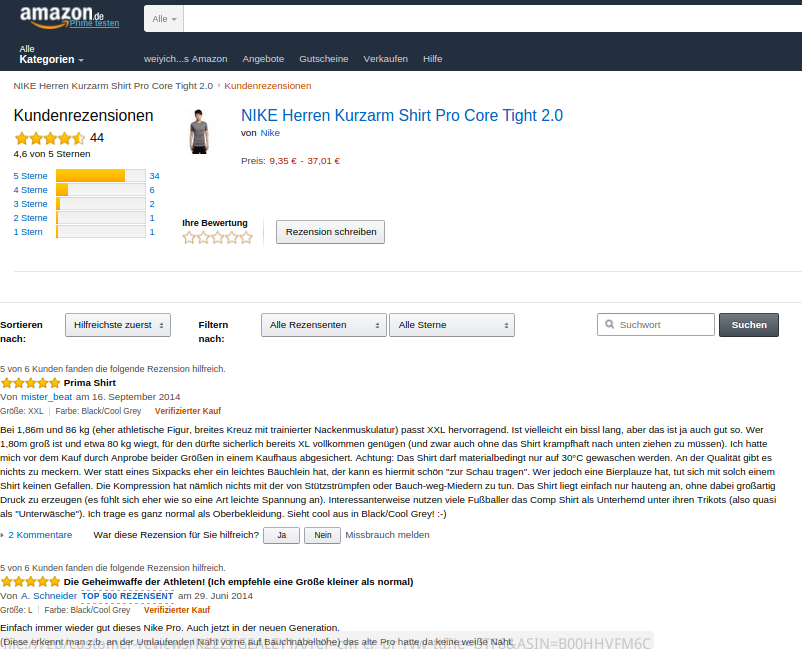
\includegraphics[scale=0.41]{datensammlung/AmazonWebseite}
	\caption[Kundenrezensionen von Amazon.de]{Kundenrezensionen von Amazon.de (Quelle: \href{http://www.amazon.de/product-reviews/B00HHVFM6C/ref=cm\_cr\_dp\_see\_all\_summary?ie=UTF8&showViewpoints=1&sortBy=byRankDescending}{Amazon.de})}
	\label{fig:AmazonSeite}
\end{figure}
Aus dem Bild kann man einfach die Struktur der Webseite verstehen. Sie ist ganz einfach: Es steht das Logo von Amazon Deutschland und die Suchleiste oben. Danach sind die Situation der Sternen, die von jedem Kunde gemacht wurde. Rechts steht der Namen und links die Ware. Darunter ist eine Tabelle, in der es alle Kundenrezensionen gibt. Jede Kundenrezension ist inklusive: Title, Sterne, Autor der Rezension, Zeitpunkt, die Kommentartexte und so weiter. Abbildung \ref{fig:AmazonStruktur} zeigt intuitiv die Struktur auf.
\begin{figure}[htb]
	\centering
		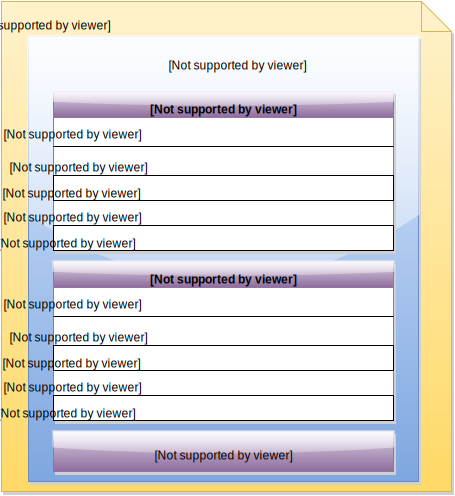
\includegraphics[scale=0.8]{datensammlung/AmazonStruktur}
	\caption[Die Struktur der Webseite von Amazon.de]{Die Struktur der Webseite von Amazon.de (Quelle: Eigene Darstellung)}
	\label{fig:AmazonStruktur}
\end{figure}

Bei der gezeigten Struktur ist der Daten-Scraping-Prozess einfach mit den obigen technischen Werkzeugen. Man kann die Tabelle von den Rezensionen lokalisieren mit folgendem Code in Python:

\code{import scrapy}

\code{table = response.xpath(`//*[@id=''productReviews'']')}

\code{.xpath()} ist eine Funktion, die von Bibliothek \emph{Scrapy} geboten wird, die XPath-Ausdrücke zu unterstützen. Dieser XPath-Ausdruck \code{//*[@id=''productReviews'']} bedeutet, dass das Element, das mit der Identität ``productReviews'' ist, selektiert wird.

\code{divs = table.xpath(`.//div[contains(@style, ''margin-left:0.5em;'')]')}

Der obige Code selektiert die Elemente, die in der Tabelle von den Rezensionen sind. Jedes selektierte Element ist ein Objekt, welches die Information von Titel, Autor, Zeitpunkt, Kommentartexte und weiteren Attributen der Rezension inklusive ist. Für jedes Element kann man mit folgendem Code die Informationen exportieren:

\code{for div in divs:} 

\code{item = AmazonItem()}

\code{item[`titel']=div.xpath(`.//span[contains(@style,\\''vertical-align:middle;'')]/b/text()').extract()} 

\code{item[`kommentartexte']=div.xpath(`.//div[@class=''reviewText'']\\/text()').extract()} 

%%\code{$item['sterne']=div.xpath('.//span[contains(@class, ''swSprite s\_star\_'')]/span/text()').extract()$} 

%%\code{$item['zeit']=div.xpath('.//span[contains(@style, ''vertical-align:middle;'')]/nobr\\/text()').extract()$} 

\code{yield item} 

Mit folgendem Bash-Code kann man alle Informationen in \emph{.json}-Dokument exportieren. Ein \emph{.json}-Dokument kann im Internet einfach ins \acs{CSV}-Dokument transformiert werden. Dann ist das Ziel der Datensammlung von Amazon Deutschland erreicht. 

\code{scrapy crawl Amazon -o items.json}
%%=============================
\subsection{Sammeln der Daten aus Tmall.com}
%%=============================
Man muss noch ein Programm in Python schreiben, um die Daten aus Tmall zu sammeln, weil Tmall und Amazon unterschiedliche Strukturen von Webseiten haben. Die folgende Abbildung \ref{fig:TmallWebseite} zeigt diese chinesischen Webseiten in Tmall.
\begin{figure}[htb]
	\centering
		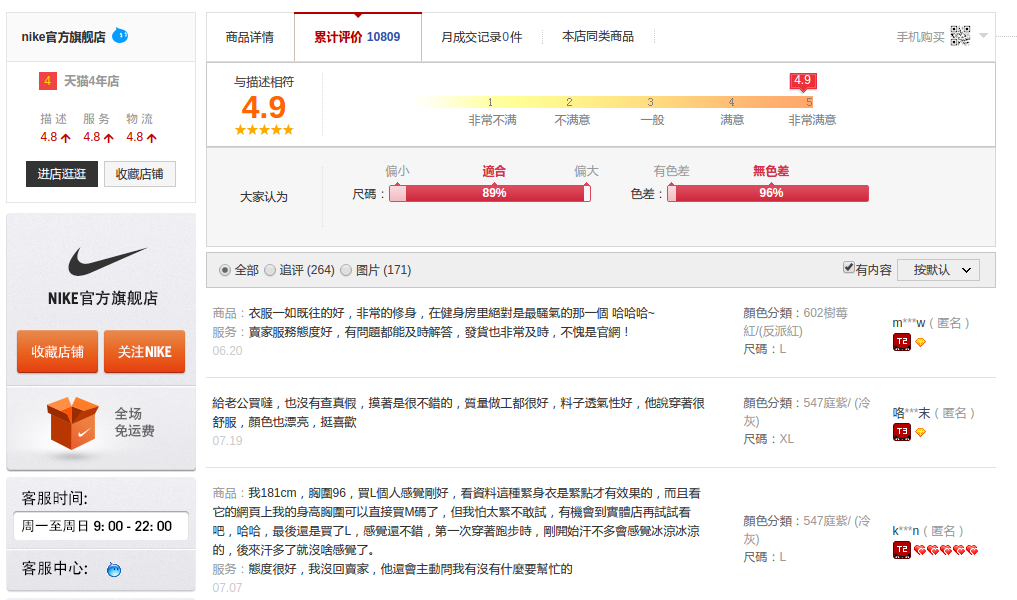
\includegraphics[width=\textwidth]{datensammlung/TmallWebseite}
	\caption[Kundenrezensionen von Tmall.com]{Kundenrezensionen von Tmall.com (Quelle: \href{http://world.tmall.com/item/21847180765.htm?spm=a1z10.5-b.w4011-2637950499.137.bsbnz1&id=21847180765&rn=2dcf6ad4e64eaaf22642aadc96bb4ab8&abbucket=9}{Tmall.com})}
	\label{fig:TmallWebseite}
\end{figure}

Es ist einfach zu finden, da alle Daten der Kundenrezensionen in einem \emph{.json}-File gespeichert sind. Deswegen braucht man nur dieses Dokument runterzuladen, und nach \acs{CSV}-Datei zu transformieren. Mit folgendem Code kann man die Daten als \emph{.json}-Datei speichern. Der regulare Ausdruck \verb;`\"rateList\":(\[.*?\])\,\"tags\"'; macht das Dokument valid.

\verb;myjson = re.findall(`\"rateList\":(\[.*?\])\,\"tags\"';\\
\verb;,myweb.text)[0].encode(`utf-8');\\
\code{f = file(`rate.json', `a')}\\
\code{f.write(myjson)}

Natürlich werden die gesammelten Daten auf chinesisch sein, weil fast alle Kunden in Tmall Chinesen sind. Um einen besseren Vergleich in dieser Arbeit zu machen, werden die chinesischen Daten ins Deutsche von Google Translater übersetzt. Dann ist das Ziel der Datensammlung aus Tmall erreicht.
%%================================================
\section{Textverarbeitung}
%%==================================================
Vor dem Start der vollwertigen Analysen müssen die aus verschiedenen Quellen erfassten Rohdaten oft eine Vorverarbeitung machen \citep{Ravi2015}. Einige in dieser Arbeit genutzten Vorverarbeitungsschritte sind:
\begin{description}
	\item[Tokenisierung:] Aufgabe zur Trennung des Volltextzeichenfolge in eine Liste von einzelnen Wörtern \citep{Balazs2016}. Es ist einfach dies in Leerzeichen getrennte Sprachen wie Englisch, Spanisch oder Deutsch durchzuführen, es wird aber wesentlich schwieriger in Sprachen in denen Wörter nicht durch Leerzeichen getrennte werden, wie Chinesisch oder Japanisch \citep[p.~9-30]{dale2000handbook}.Deshalb werden die Rohdaten von Tmall erst nach Deutsch übersetzt, und dann werden die Vorverarbeitungsschritte gemacht. Mit folgendem Code in R kann man diesen Schritt erledigen:

	\verb;word.list = str_split(sentence, `\\s+');
	\item[Stemming:] heuristische Verfahren zum Löschen von Wort Affixen und verlassen sie in einer invarianten kanonischen Form oder ``\acs{i.e.} stem'' \citep{Balazs2016}. Zum Beispiel: Einkauf, Einkaufen, einkaufen werden als ``Einkauf'' gestemmt.Dieser Schritt wird in R so fertig gemacht:

	\verb;docs <- tm_map(docs,stemDocument,language="german");
	\item[Stoppwörtern Entfernen:] Aktivität zum Entfernen von Wörtern, die für die Strukturierung von Sprache verwendet werden, aber leisten keinen Beitrag zum Inhalt \citep{Balazs2016}. Einige dieser Wörter sind wie zum Beispiel: die, war, oder wird. In R wird es so gemacht:

	\verb;docs <- tm_map(docs, removeWords, stopwords("german"));

	Und man kann auch selbst einige Stoppwörter definieren. Zum Beispiel: beim, im, oder schon mit solchem Code: 

	\verb;docs <- tm_map(docs, removeWords, c("schon", "beim"));
%%	\item[Wortart Tagging:] (\acs{i.e.} \ac{POS} Tagging). In dem Schritt wird jedes Wort eines Satzes mit der Wortart gekennzeichnet, wie Adjektiv, Substantiv, Verb, Adverb und Präposition \citep{Brill:1992:SRP:974499.974526}.
	\item[Sonstiges Entfernen oder Änderungen:] wie zum Beispiel: in Kleinbuchstaben umwandeln, die Zahlen und Satzzeichen entfernen. Mit folgendem Code werden sie beschäftigt:

	\verb;docs <- tm_map(docs, removeNumbers);\\
	\verb;docs <- tm_map(docs, content_transformer(tolower));\\
	\verb;docs <- tm_map(docs, removePunctuation);
\end{description}
%%================================	
Nur mit diesen Vorverarbeitungsschritten können die Analysen in dieser Arbeit ausgeführt werden. Nach diesen Schritten werden die Vorbereitungen der Daten für die Analysen in dieser Arbeit geschaffen.
%%====================================
\section{Maschinelle Übersetzung für mehrsprachige Sentiment-Analyse} \label{mehrsprachig}
%%====================================
Vor dem Beginn der Analyse, muss man erkennen, dass die in dieser Arbeit gemachte kulturübergreifende Sentiment-Analyse eine mehrsprachige (Deutsch und Chinesisch) Analyse ist. Mit vielen Rohdaten, muss man in dieser Arbeit eine maschinelle Übersetzung machen. Deswegen werden die chinesischen Kommentaren ins Deutsche durch Google Translate übersetzt. In diesem Abschnitt wird diskutiert, ob die originalen Daten nach der maschinellen Übersetzung noch valid und zuverlässig sind.

Es gab schon in der Praxis einige Forschungen , die maschinelle Übersetzung für mehrsprachige Sentiment-Analyse benutzen, zum Beispiel: \citet{demirtas2013cross} machte eine mehrsprachige Sentiment-Analyse zwischen Türkisch und Englisch, bei der Google Translate für die türkischen \ac{OCRs} von Filmen und verschiedenen Produkten benutzt wurde. \citet{Scholz2012} benutzten auch Google Translate für die fünfsprachige Sentiment-Analyse (Italienisch, Spanisch, Französisch, Deutsch und Englisch). \citet{Momtazi2012} machte die Forschung von der deutschsprachigen Sentiment-Analyse auch mit Google Translate.

Andererseits machen die Wissenschaftler noch einige theoretische Grundlagen für die maschinelle Übersetzung. \citet{Balahur2014} haben herausgefunden, dass die Übersetzungsmaschine einen angemessenen Reifegrad erreichen muss, um ausreichend zuverlässige Daten für andere Sprachen zu produzieren. Die Lücke in der Klassifikationsleistung zwischen auf Englisch geschulten Systemen und übersetzten Daten ist minimal, mit einem Maximum von 11.8\% zugunsten der Ausgangssprachesdaten. Experimentelle Ergebnisse von \citet{Wan2008} zeigen, dass die Analyse der Reviews auf Englisch, die durch die Übersetzungsdienst (zum Beispiel: Google Translate und Yahoo Babel Fish) übersetzt werden, an Leistung übertrifft, als die Analyse der ursprünglichen chinesischen Reviews.

In dieser Arbeit, werden die chinesischen Kommentaren auf Deutsch durch Google Translate übersetzt. Es wird wenige Einflüsse geben, nicht nur wegen den Ergebnissen von Praxis- und Theorieseiten, sondern auch wegen den folgenden Gründen:
\begin{enumerate}
	\item Wie in Abschnitt \ref{algorithmus} gesagt, wird das Lexikon von \citet{Remus2010} in dieser Arbeit verwendet. Dieses Lexikon nach \citet{Remus2010} wird auch teilweise durch Google Translate von Englisch auf Deutsch übersetzt. 
	\item Nach der Textverarbeitung, werden die Rohdaten in den einzeln Wörtern getrennt, und in eine invariante kanonischen Form gestellt. Das heißt: die Reihenfolge des Satzes und Formen der Wörtern sind nicht wichtig. Zum Beispiel, es gibt solche Kommentare in Chinesisch:

	\begin{CJK*}{UTF8}{gbsn}
	东西很好,昨天穿了刚刚好!我180、74kg!很不错,就是客服比较傲,经常不回复。
	\end{CJK*}

	Der Kunde meint: 

	\emph{Die Dinge sind gut, ich habe sie gestern angezogen, genau das Richtige! Ich bin 180cm groß, wiege 74kg. Sehr gut, aber der Mitarbeiter des Kundendiensts ist relativ stolz, weil er oft nicht auf mich reagiert.}

	Durch Google Translate: 

	\emph{Etwas Gutes gestern, tragen genau das Richtige! Ich 180,74kg! Sehr gut, ist es relativ stolz auf die Kunden-Service, die oft nicht reagieren.}

	Nach der Textverarbeitung werden nur die Wörtern behalten:
	
	\begin{CJK*}{UTF8}{gbsn}
	\begin{table}[h]
	\centering
	\begin{tabular}{lllll}
	\hline
	Chinesisch       & 好  & 刚刚好        & 不错& 傲 \\ \hline
	Deutsch          & gut & genau richtig & gut & stolz \\ \hline
	Google Translate & gut & genau richtig & gut & stolz \\ \hline
	\end{tabular}
	\caption[Vergleich zwischen manueller und maschineller Übersetzung nach der Textverabeitung]{Vergleich zwischen manueller und maschineller Übersetzung nach der Textverabeitung (Quelle: eigene Darstellung)}
	\label{tab:maschinelleÜbersetzung}
	\end{table}
	\end{CJK*}

Durch Tabelle \ref{tab:maschinelleÜbersetzung} kann man deutlich sehen, dass die Übersetzungsergebnisse von Maschine oder vom Menschen gleich oder fast gleich sind. Verglichen mit der manuellen Übersetzung, macht sich die Maschine schon gut genug für die Forschung, und es ist schneller und kostet weniger. Aus diesen Gründen macht Google Translate die Übersetzung in dieser Arbeit.
\end{enumerate}
